\documentclass[a4paper,9pt,twocolumn]{extarticle}
\usepackage[pdftex]{color,graphicx}
\usepackage{assets/include/elaboration}

\onecolumn
\mywork{}{Your ID}{An LLM-Based Bilingual Campus Assistant for Academic Service Access via RAG and Quiizy Integration: Design, Implementation, Cloud Deployment and Evaluation in a Central African University}
\mycoauthors{
Moutcheu Somo Gift Anderson\\
Abena Alex Nelson Ryan\\
Foning Lackmata Luc-Xavier\\
Fotsing Kengne Weber\\
Chengho Fongang Marie Louise\\
Kouetche Simo Yann\\
Takam Sokoudjo Ismael Ulrich
}
\mydate{March 29, 2026}

\usepackage[hypertexnames=false,hidelinks,pdftex,
            pdfauthor={\MyAuthor},
            pdftitle={\MyThema},
            pdfsubject={Scientific Document}]{hyperref}

\begin{document}
\mytitle

\newpage
\vspace*{\stretch{1}}
\noindent
Supervisor:\\
Dr.-Ing. Philippe Tamla\\
Professor for Data Science and Artificial Intelligence\\
PostDoc Researcher at\\
Department of Multimedia and Internet Applications\\
Faculty of Mathematics und Computer Science\\
Universit\"atsstr. 1\\
58097 Hagen\\
\vfil\null

\newpage
\section*{Abstract}
This paper presents the design, implementation, and evaluation of a
web-based Smart Campus AI Assistant for university students. Leveraging a
\textbf{Large Language Model (LLM)} and a \textbf{Retrieval-Augmented Generation (RAG)}
pipeline, the system provides bilingual academic and administrative
service access within a Central African university context. The assistant
is designed to integrate with \textbf{Quiizy}, an academic platform used for
student multiple-choice assessments and related course information
access. The research follows the Nunamaker methodology and evaluates the
system through a \textbf{Cognitive Walkthrough (CW)} and a student satisfaction
survey grounded in the \textbf{Technology Acceptance Model (TAM)}.

\newpage
\tableofcontents
\newpage
\listoffigures
\newpage
\listoftables
\newpage
\listoflistings
\newpage
\twocolumn
\mainmatter

\section{Introduction}
\label{sec:intro}

Universities in developing countries increasingly rely on web-based
digital services to support students. Typical services include
retrieving academic information, for example course details and
announcements, completing administrative tasks, finding schedules, and
getting study support. As enrolment grows and support offices remain
limited, students often face long response times and fragmented
information sources. Across Africa, these difficulties are intensified
by infrastructure constraints and uneven access conditions. In Cameroon,
they are further amplified by a bilingual academic environment in which
students may need the same service in both English and French. To make
such services available at scale, universities increasingly host
applications on cloud computing platforms such as Amazon Web Services
(AWS). In this paper, cloud computing means delivering computing
resources such as servers, storage, and databases over the internet on
demand, rather than running and maintaining all infrastructure locally
\cite{shukur2020cloud,rashid2018distributed}.

This work focuses on a web-based campus assistant for student services.
In this paper, the assistant is powered by \textbf{Artificial Intelligence
(AI)}, meaning computer methods that can perform tasks that normally
require human intelligence such as language understanding. We therefore
refer to the system as a \textbf{Smart Campus AI Assistant}: a web-based
student support system that answers questions and helps students reach
campus services through natural-language dialogue. A key component is a
\textbf{Large Language Model (LLM)}, a deep-learning model trained on large
text collections that can generate fluent text responses
\cite{zhao2023survey,brown2020language}. When an LLM is placed inside a
dialogue interface it becomes a conversational agent, or chatbot, which
interacts with users through conversation instead of menus
\cite{labadze2023,pereira2023}. Effective campus assistants often need
more than question-answering. This paper therefore also uses a
\textbf{Retrieval-Augmented Generation (RAG)} pipeline, which combines
generation with retrieval by first searching a verified document
collection and then generating an answer using the retrieved passages as
evidence \cite{lewis2020retrieval,gao2023retrieval}. The assistant is
also designed to connect to \textbf{Quiizy}, the academic platform in the
target institution through which students take multiple-choice tests and
access related course information. This explicit platform scope is
retained to satisfy the reviewer comment asking which specific assistant
and which concrete LMS-like integration are being addressed.

\textbf{MS1: Smart campus systems can improve student engagement when they
make academic information easier to access and use.} Student engagement
is understood here as students' effective interaction with academic
resources, deadlines, and support services needed for their studies.
Evidence suggests that smart campus systems embedding AI services can
improve engagement by reducing information friction and making
institutional resources more responsive \cite{chen2024}. \textbf{MS2:
AI-based campus assistants require rigorous usability and acceptance
evaluation before they can be considered genuinely helpful.} Response
delay in this paper refers to the time students experience between
requesting information and obtaining a useful answer, whether from human
staff or digital systems. Reducing this delay matters only if the
system is also understandable, learnable, and trusted, which is why
usability and acceptance evaluation remain central
\cite{hollingsed2007,mahatody2010,davis1989}.

The overall goal of this research is to design, implement, and evaluate
a web-based Smart Campus AI Assistant that provides bilingual academic
and administrative support using an LLM-based conversational interface,
a RAG-based retrieval component, and integration with the Quiizy
platform context. Based on this goal, the research addresses two
problems. \textbf{PS1:} The existing literature provides limited evidence
of well-documented and evaluated bilingual campus assistants for Central
African universities that ground their answers in institutional sources
through an LLM plus a retrieval component
\cite{labadze2023,pereira2023,lewis2020retrieval,gao2023retrieval}.
\textbf{PS2:} Even when prototypes exist in other regions, many studies
rely on informal feedback or omit structured usability inspection and
acceptance models. As a result, it can be difficult to assess whether
the systems are easy to learn and useful for students
\cite{hollingsed2007,mahatody2010,davis1989,venkatesh2003,delone2003}.
These problems connect directly to the introduction because they explain
why the proposed system must be both context-specific and rigorously
evaluated, making the research intent explicit and easy to follow.

These motivations lead to two research questions. \textbf{RQ1:} How can a
web-based Smart Campus AI Assistant that integrates an LLM, a
RAG-enabled retrieval component, and Quiizy-linked academic content be
designed, implemented, and deployed on a cloud computing platform to
provide bilingual academic service access for university students?
\textbf{RQ2:} To what extent does the implemented assistant meet usability
expectations, and how does it affect student satisfaction and access to
academic information?

This research follows the well-established Nunamaker systems development
research framework \cite{nunamaker1991}, a structured approach for
developing information systems consisting of four phases:
\textbf{Observation}, \textbf{Theory Building}, \textbf{Implementation}, and
\textbf{Experimentation}. Following this methodology, the research
objectives are grouped by research question and expressed in the
Nunamaker categories of Observation (\textbf{O}), Theory Building
(\textbf{TB}), Implementation (\textbf{I}), and Experiment
(\textbf{E}). The objectives related to \textbf{RQ1} are as follows:
\textbf{RO1.1--O:} Review existing methods and tools for AI chatbots,
conversational agents, LLMs, RAG architectures, cloud deployment, and
platform integration in higher education, especially in developing and
multilingual contexts. \textbf{RO1.2--TB:} Derive the design requirements
and system model for a Smart Campus AI Assistant based on an LLM, a
RAG-enabled retrieval pipeline, cloud deployment support, and
integration with Quiizy. \textbf{RO1.3--I:} Implement a bilingual
web-based prototype that supports English and French interaction for
academic service access and deploy on AWS cloud infrastructure. \textbf{RO1.4--E:} Evaluate whether the
implemented prototype improves access to academic information and task
support for representative student use cases. The objectives related to
\textbf{RQ2} are as follows: \textbf{RO2.1--O:} Review usability issues,
interaction challenges, and student expectations relevant to AI-based
educational assistants. \textbf{RO2.2--TB:} Define an evaluation model
grounded in usability, technology acceptance, and information systems
success theory. \textbf{RO2.3--I:} Instrument the prototype and
evaluation materials so that usability and student-satisfaction data can
be collected systematically. \textbf{RO2.4--E:} Conduct a usability
inspection and student satisfaction study to assess learnability,
perceived usefulness, perceived ease of use, and overall service
quality.

To answer the research questions, the study proceeds in a simple and
traceable way. Observation activities identify the student
information-access constraints and bilingual service needs. Theory
building translates these into system and evaluation requirements.
Implementation realises a bilingual web prototype, and experimentation
assesses whether the resulting artefact is usable and useful enough to
address the original problems. The remainder of this paper is organised
as follows. Chapter 2 reviews related work on conversational agents in
higher education, LLMs, RAG, platform integration, and evaluation
frameworks. Chapter 3 presents the system design and modelling. Chapter
4 describes the implementation. Chapter 5 reports evaluation results.
Chapter 6 concludes with limitations and future work. Chapter 2 is
structured to support the design choices made later in the paper: it
surveys chatbot use in universities, reviews LLM foundations and
limitations, introduces RAG for grounded institutional question
answering, analyses LMS and platform integration patterns, compares
related university assistant systems, and summarises evaluation
frameworks combining usability inspection and acceptance models.

\section{State of the Art in Science and Technology}
\label{sec:soa}

This chapter presents the state of the art in scientific and
technological approaches directly relevant to the design and evaluation
of a web-based, bilingual, LLM-based campus assistant integrated with an
academic platform for university students in a Central African context.
The review supports the observation phase of the Nunamaker methodology
\cite{nunamaker1991} and specifically addresses research objectives
RO1.1--O and RO2.1--O by documenting student information-access needs,
surveying relevant technological solutions, and identifying their
limitations.

The chapter is organised as follows. Section 2.1 surveys AI chatbots and
conversational agents in higher education. Section 2.2 examines LLMs as
the enabling technology for natural language understanding and
generation. Section 2.3 presents RAG as the principal architectural
approach for grounding responses in verified institutional knowledge.
Section 2.4 analyses chatbot integration with learning and assessment
platforms, including the type of functionality represented here by
Quiizy. Section 2.5 reviews comparable university AI assistant systems.
Section 2.6 discusses evaluation frameworks suitable for AI-based
educational systems. Based on this review, Section 2.7 formulates the
remaining challenges that motivate the modeling in Chapter 3.

\subsection{AI Chatbots and Conversational Agents in Higher Education}
\label{sec:soa:chatbots}

This section addresses RO1.1--O by reviewing AI-powered conversational
agents in higher education and establishing the documented service needs
that motivate the proposed system. A conversational agent, or chatbot,
is a software system designed to simulate human-like dialogue through a
natural-language interface, allowing users to query information, request
services, or receive guidance without navigating complex administrative
workflows \cite{labadze2023,pereira2023}. These systems range from
rule-based assistants that match input to predefined responses to more
advanced LLM-powered agents capable of multi-turn dialogue, contextual
interaction, and broader language understanding \cite{wang2024,
stoehr2024}.

Labadze et al. \cite{labadze2023} synthesize empirical evidence from
higher education and conclude that AI chatbots can significantly improve
student access to academic information by providing immediate and
personalized support. Pereira-Molina et al. \cite{pereira2023} similarly
report improvements in information accessibility and student
satisfaction, while also noting that most published deployments are
concentrated in North American and European settings. Wang et al.
\cite{wang2024} further show that conversational interfaces can reduce
administrative overhead and improve information accessibility,
particularly where human support capacity is limited.

St\"ohr et al. \cite{stoehr2024} study student perceptions of AI chatbots
and show that continued usage is closely tied to perceived response
quality and linguistic accessibility. Nguyen et al.
\cite{nguyenRoleDesign2023} argue that conversational systems should not
be limited to reactive question answering, but should instead support
goal-directed student tasks and multi-step interaction. This is directly
relevant to the current study, since students using an assistant for
Quiizy-related information may need both factual retrieval and procedural
guidance.

Despite this growing body of work, most reported campus assistants are
monolingual, domain-restricted, and evaluated in relatively stable
digital environments. Published studies on multilingual academic
assistants designed and rigorously evaluated for Central African
universities remain limited. This gap is especially important where
English and French coexist in institutional communication and where
access conditions may be uneven. We therefore identify the first
remaining challenge:

\textbf{RC1:} Existing research offers limited evidence of bilingual,
context-aware AI campus assistants designed and evaluated for Central
African university settings.

\subsection{Large Language Models for Natural Language Understanding}
\label{sec:soa:llm}

This section supports RO1.2--TB by reviewing LLMs as the core enabling
technology for natural language understanding and generation in the
proposed assistant. An LLM is a neural language model with very large
numbers of trainable parameters, pre-trained on massive text corpora to
acquire broad linguistic competence and general reasoning ability
\cite{zhao2023survey,brown2020language}. These models are particularly
well suited to dialogue systems because they can interpret open-ended
user questions and produce coherent natural-language answers.

The architectural foundation of most contemporary LLMs is the
Transformer, introduced by Vaswani et al. \cite{vaswani2017attention}.
Its self-attention mechanism allows efficient modeling of contextual
dependencies across a sequence, which is essential for understanding
complex, multi-clause student questions. Brown et al.
\cite{brown2020language} demonstrated that sufficiently scaled language
models exhibit strong few-shot behavior, which is valuable in academic
service environments where it is impossible to enumerate every possible
student query in advance.

Related model families further support the ecosystem around LLM-enabled
assistants. Devlin et al. \cite{devlin2019bert} contributed dense
language representations through BERT, which remain influential in
semantic retrieval and embedding pipelines, while Touvron et al.
\cite{touvron2023llama} expanded access to high-quality open foundation
models through LLaMA. Together, these developments make it technically
feasible to build assistants that combine generation, retrieval, and
context management.

However, LLMs also have serious limitations in institutional service
settings. First, they may hallucinate by producing fluent but incorrect
or fabricated statements \cite{zhao2023survey,gao2023retrieval}. Second,
their knowledge is static: they do not automatically reflect changes in
course content, deadlines, announcements, or platform usage rules unless
connected to external information sources \cite{lewis2020retrieval,
soliman2025rag}. These limitations are critical for an assistant that
must provide dependable academic information. This leads to the second
remaining challenge:

\textbf{RC2:} LLMs alone are insufficient for reliable institutional
information access because hallucination and static knowledge must be
addressed through external grounding mechanisms.

\subsection{Retrieval-Augmented Generation for Institutional Knowledge Access}
\label{sec:soa:rag}

This section continues RO1.2--TB by presenting RAG as the main
architectural approach for addressing the limitations identified above.
Lewis et al. \cite{lewis2020retrieval} introduced RAG as a framework
that combines parametric model knowledge in an LLM with non-parametric
knowledge retrieved from an external document collection at inference
time. In a typical RAG pipeline, a user query is transformed into a
vector representation, matched against an indexed document store, and
the most relevant passages are then supplied to the generator as context
for answer production.

For campus assistants, this architecture is especially attractive because
it allows answers to be grounded in current institutional sources rather
than in the model's internal memory alone. Gao et al.
\cite{gao2023retrieval} classify RAG systems into increasingly advanced
forms, ranging from basic retrieval-plus-generation pipelines to modular
systems that support query rewriting, reranking, and multi-step
reasoning. Essel et al. \cite{essel2025rag} show that in educational
applications, RAG improves factual accuracy, response relevance, and
user satisfaction when compared with pure LLM baselines. Soliman et al.
\cite{soliman2025rag} further argue that RAG is particularly effective in
educational settings because it addresses hallucination, knowledge
staleness, and the need for domain-specific grounding.

In the context of this paper, RAG is the mechanism through which the
assistant can use Quiizy-related and institutional content to answer
questions about quizzes, schedules, announcements, and related academic
procedures. The approach supports the reviewer's request to clarify that
the proposed intelligent component is not just an abstract autonomous
agent, but a concrete RAG-based retrieval and answer-generation
pipeline. At the same time, deployments in multilingual and
resource-constrained African educational contexts remain limited. This
supports the third remaining challenge:

\textbf{RC3:} RAG is well suited to institutional knowledge access, but
published evidence on bilingual RAG deployments adapted to Central
African university conditions remains limited.

\subsection{Integration of AI Chatbots with Learning and Assessment Platforms}
\label{sec:soa:lms}

This section addresses RO1.1--O and RO1.2--TB by reviewing the
integration of AI chatbots with learning and assessment platforms such as
LMS environments and the Quiizy platform targeted in this study.
Platforms of this kind manage course materials, assignments, assessment
activities, grades, announcements, and related student-facing services.
When a conversational assistant is connected to such a platform, it can
support personalized, real-time queries that depend on institutional
data rather than static general knowledge \cite{alsaqqa2025,neumann2025,
kim2025}.

Al-Saqqa et al. \cite{alsaqqa2025} show that chatbot integration varies
in both technical depth and personalization depth. Many existing systems
remain at the level of document ingestion, without exploiting the richer
student-specific context available through platform data. Neumann et al.
\cite{neumann2025} demonstrate that an LLM-driven chatbot integrated with
an educational information environment can improve access to relevant
course content through retrieval and contextual dialogue. Kim et al.
\cite{kim2025} further show that memory-augmented language-model
architectures can preserve conversational context across multiple turns,
which is important when students ask follow-up questions about ongoing
tasks or deadlines.

For this study, the relevant integration context is Quiizy, a platform
used for student multiple-choice tests and related academic information.
The proposed assistant therefore targets a concrete, bounded service
domain rather than a generic or unspecified LMS. This directly answers
the PDF comments requesting that the paper name the platform and the
specific services under discussion. Even so, published reports of
RAG-enabled assistants designed and evaluated for platform ecosystems of
this kind in Francophone or bilingual Central African universities remain
rare. This motivates the fourth remaining challenge:

\textbf{RC4:} Platform-integrated educational assistants are promising,
but comparable bilingual solutions designed for Quiizy-like academic
environments in Central African universities remain underexplored.

\subsection{Comparable University AI Assistant Systems}
\label{sec:soa:systems}

This section supports RO1.1--O and anticipates RO1.4--E by reviewing
comparable university AI assistant systems. Several prior systems
demonstrate technical feasibility, but each leaves open aspects that are
central to the present study.

Akiba and Fraboni \cite{akiba2023} discuss AI-supported academic advising
through large language models and show the growing potential of such
systems to support student empowerment. Nguyen et al.
\cite{nguyen2024unibot} present a document-retrieval chatbot for
education settings that integrates information retrieval with an LLM and
reports strong relevance performance. Neupane et al.
\cite{neupane2024} likewise demonstrate that indexing heterogeneous
university resources into a retrieval pipeline can reduce hallucination
and improve answer usefulness.

In multilingual settings, Bilquise et al. \cite{bilquise2022} show that
a bilingual academic-advising chatbot can expand reach and improve
perceived usefulness for non-English-speaking student populations. This
is an important methodological precedent for the English-French design
required in Cameroon. Tamascelli et al. \cite{tamascelli2025} further
show that agent-supported academic advising systems can outperform
purely retrieval-based interfaces on more complex student tasks.

Taken together, these systems confirm that LLM-based university
assistants are feasible and useful. However, few combine all of the
requirements relevant here: bilingual English-French interaction,
RAG-grounded answers, integration with an academic platform such as
Quiizy, cloud deployment considerations, and a combined usability and
acceptance evaluation in a Central African context. This motivates the
fifth remaining challenge:

\textbf{RC5:} Comparable university AI assistant systems demonstrate
feasibility, but not the full combination of bilingualism, RAG grounding,
platform integration, and Central African evaluation required here.

\subsection{Evaluation Frameworks for AI-Based Educational Systems}
\label{sec:soa:evaluation}

This section addresses RO2.1--O and supports RO2.2--TB by reviewing the
evaluation frameworks employed in this research. Evaluating an AI campus
assistant requires capturing both technical behavior and user-centered
experience. Relevant dimensions include response quality, retrieval
faithfulness, learnability, perceived usefulness, ease of use, and
overall student satisfaction.

The \textbf{Cognitive Walkthrough (CW)} is a scenario-based usability
inspection method in which evaluators step through tasks to determine
whether a system is understandable and learnable without prior training.
Hollingsed and Novick \cite{hollingsed2007} show that CW reliably reveals
learnability problems in goal-oriented interactive systems. Mahatody et
al. \cite{mahatody2010} further classify the evolution of the method and
confirm its continued relevance as a cost-effective inspection technique.
Because chatbot systems rely heavily on user formulation of requests and
system guidance, CW is well suited to identifying interaction breakdowns
before large-scale user testing.

For user acceptance, the \textbf{Technology Acceptance Model (TAM)}
proposed by Davis \cite{davis1989} remains foundational. TAM centers on
perceived usefulness and perceived ease of use as key determinants of
technology adoption. Venkatesh et al. \cite{venkatesh2003} extend this
line of thinking through UTAUT, adding factors such as social influence
and facilitating conditions. DeLone and McLean
\cite{delone2003} contribute a complementary information-systems success
perspective through information quality, system quality, and service
quality.

Used together, these frameworks provide a strong basis for evaluating
whether the proposed assistant is not only technically functional but
also understandable, useful, and acceptable to students. Yet combined
evaluation protocols of this kind remain uncommon for bilingual,
RAG-enabled, platform-integrated campus assistants in Central African
contexts. This supports the sixth remaining challenge:

\textbf{RC6:} A rigorous combined evaluation framework is available, but
it has rarely been applied to bilingual, RAG-based campus assistants in
the target context.

\subsection{Summary and Research Gap}
\label{sec:soa:gap}

This chapter has reviewed the principal scientific and technological
foundations of the proposed Smart Campus AI Assistant. Section 2.1
showed that AI chatbots can improve academic information access, but
bilingual Central African deployments remain rare (RC1). Section 2.2
established that LLMs provide strong natural-language capabilities but
must be augmented to avoid hallucination and stale knowledge (RC2).
Section 2.3 demonstrated that RAG is an appropriate grounding mechanism
for institutional knowledge access, but context-specific bilingual
deployments remain limited (RC3). Section 2.4 confirmed the value of
integrating assistants with learning and assessment platforms such as
Quiizy, while also revealing the scarcity of evaluated solutions in the
target context (RC4). Section 2.5 showed that comparable systems confirm
feasibility without fully matching the combination of requirements in
this study (RC5). Section 2.6 identified a suitable combined evaluation
framework while also showing that it has rarely been applied in this
specific setting (RC6).

Taken together, these six remaining challenges define a coherent
research space: the design, implementation, deployment, and evaluation
of a bilingual, RAG-enabled, Quiizy-integrated Smart Campus AI Assistant
for a Central African university. These findings directly motivate the
modeling choices developed in the next chapter.

\section{Design and Modeling}
\label{sec:model}

This chapter presents the proposed system design (Theory Building in the
Nunamaker methodology \cite{nunamaker1991}). The design is guided by
\textbf{User-Centered Design (UCD)}: the architecture is derived from the
users' tasks and constraints (mobile-first access, bilingual interaction,
and limited human support capacity), and only then mapped to concrete
technology components.

The proposed artefact extends the existing Quiizy platform with a
bilingual (English/French) conversational assistant for academic service
access. Answers are grounded in institutional course documents through
\textbf{RAG} (Retrieval-Augmented Generation): the system retrieves relevant
passages from a trusted document collection and uses these passages as
context when generating the response.

To remain concise, technical terms are used sparingly and in a pragmatic
way. A \textbf{webhook} is an HTTP endpoint that receives events (here:
WhatsApp messages). An \textbf{embedding} is a numeric representation of
text meaning, and a \textbf{vector store} is a database that stores
embeddings to support similarity search.

\subsection{The Existing System and the Design Context}
\label{sec:model:context}

The platform being extended is Quiizy, a web-based academic assessment
system implemented with NestJS (Node.js) and backed by PostgreSQL
\cite{nestjsDocs,postgresDocs}. The data-access layer uses TypeORM
\cite{typeormDocs}. The existing authentication mechanism relies on JWT
(a signed token used to represent an authenticated session).

Rather than replacing Quiizy, the design adds three capabilities that map
directly to user needs:
(1) a teacher-facing workflow to upload course materials within the LMS,
(2) a document indexing pipeline that makes uploaded materials searchable
by meaning (RAG), and (3) a student-facing conversational interface that
returns responses in English or French.

Note that Quiizy includes a native mobile application for students to take quizzes;
this mobile app is already implemented and is outside the scope of the present research.
The research focuses exclusively on the web-based conversational assistant interface
for academic service access.

In UCD terms, the primary requirement is to minimise user effort while
maximising access speed and clarity: students interact through a conversational
interface, teachers use a small extension of the existing web workflow, and the
retrieval infrastructure remains lightweight enough to deploy within constrained
institutional environments.

\subsection{Use Case Model}
\label{sec:model:usecase}

Figure \ref{fig:use-case-model} shows the use case model with four actors:
Student, Teacher, Administrator, and an \textbf{IR Agent}.
Here, \textbf{IR Agent} denotes the retrieval component responsible for
selecting relevant passages from the indexed course documents.

\begin{figure*}[htbp]
  \centering
  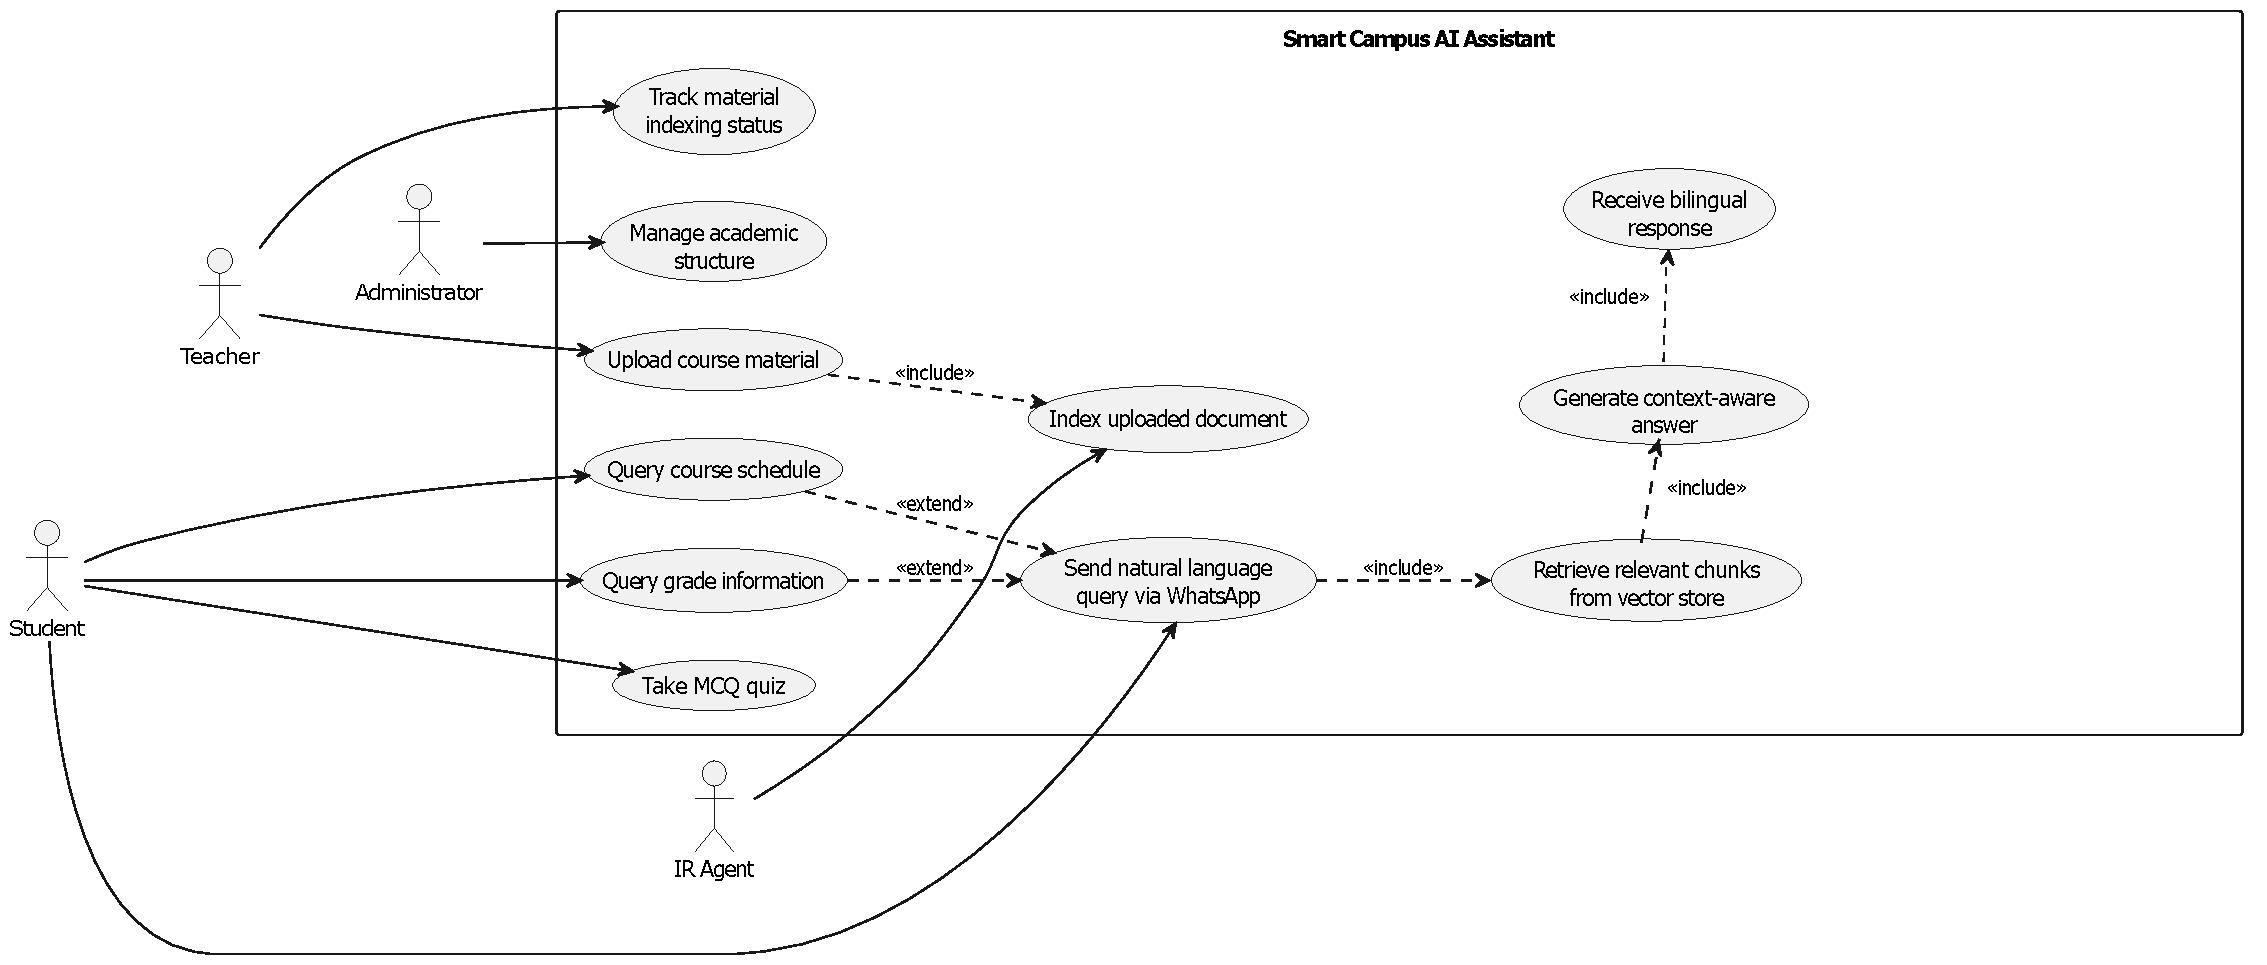
\includegraphics[width=1.06\textwidth]{images/UseCase.pdf}
  \caption{Use case diagram of the Smart Campus AI Assistant}
  \label{fig:use-case-model}
\end{figure*}

The student's primary use case is to ask a natural-language question through
the conversational interface and receive a grounded answer in the language of the request.
Internally, the system executes a short pipeline: (a) retrieve relevant
document passages, (b) assemble a prompt that includes the retrieved
context, and (c) generate the final response using the LLM.

The teacher's primary use case is to upload course materials through the
web interface. The system then extracts text and indexes it for later
retrieval. The administrator continues to manage the academic structure
in Quiizy without changes; the assistant features are additive.

\begin{figure*}[htbp]
  \centering
  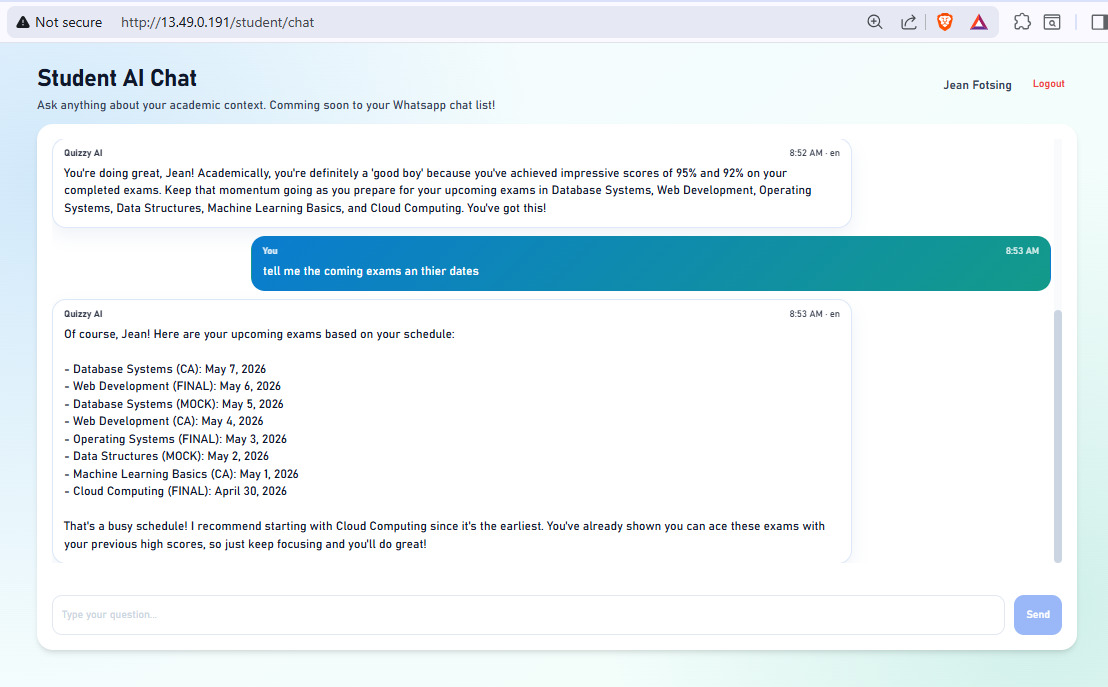
\includegraphics[width=0.95\textwidth]{images/quiizy_student_chat.png}
  \caption{Web-based conversational interface for student academic service access}
  \label{fig:student-chat-interface}
\end{figure*}

\subsection{System Architecture}
\label{sec:model:architecture}

The overall architecture is shown in Figure \ref{fig:component-architecture}.
The existing Quiizy backend stays in place, and new components are added
around it for (1) document upload and indexing and (2) conversational chat
services.

\begin{figure*}[htbp]
  \centering
  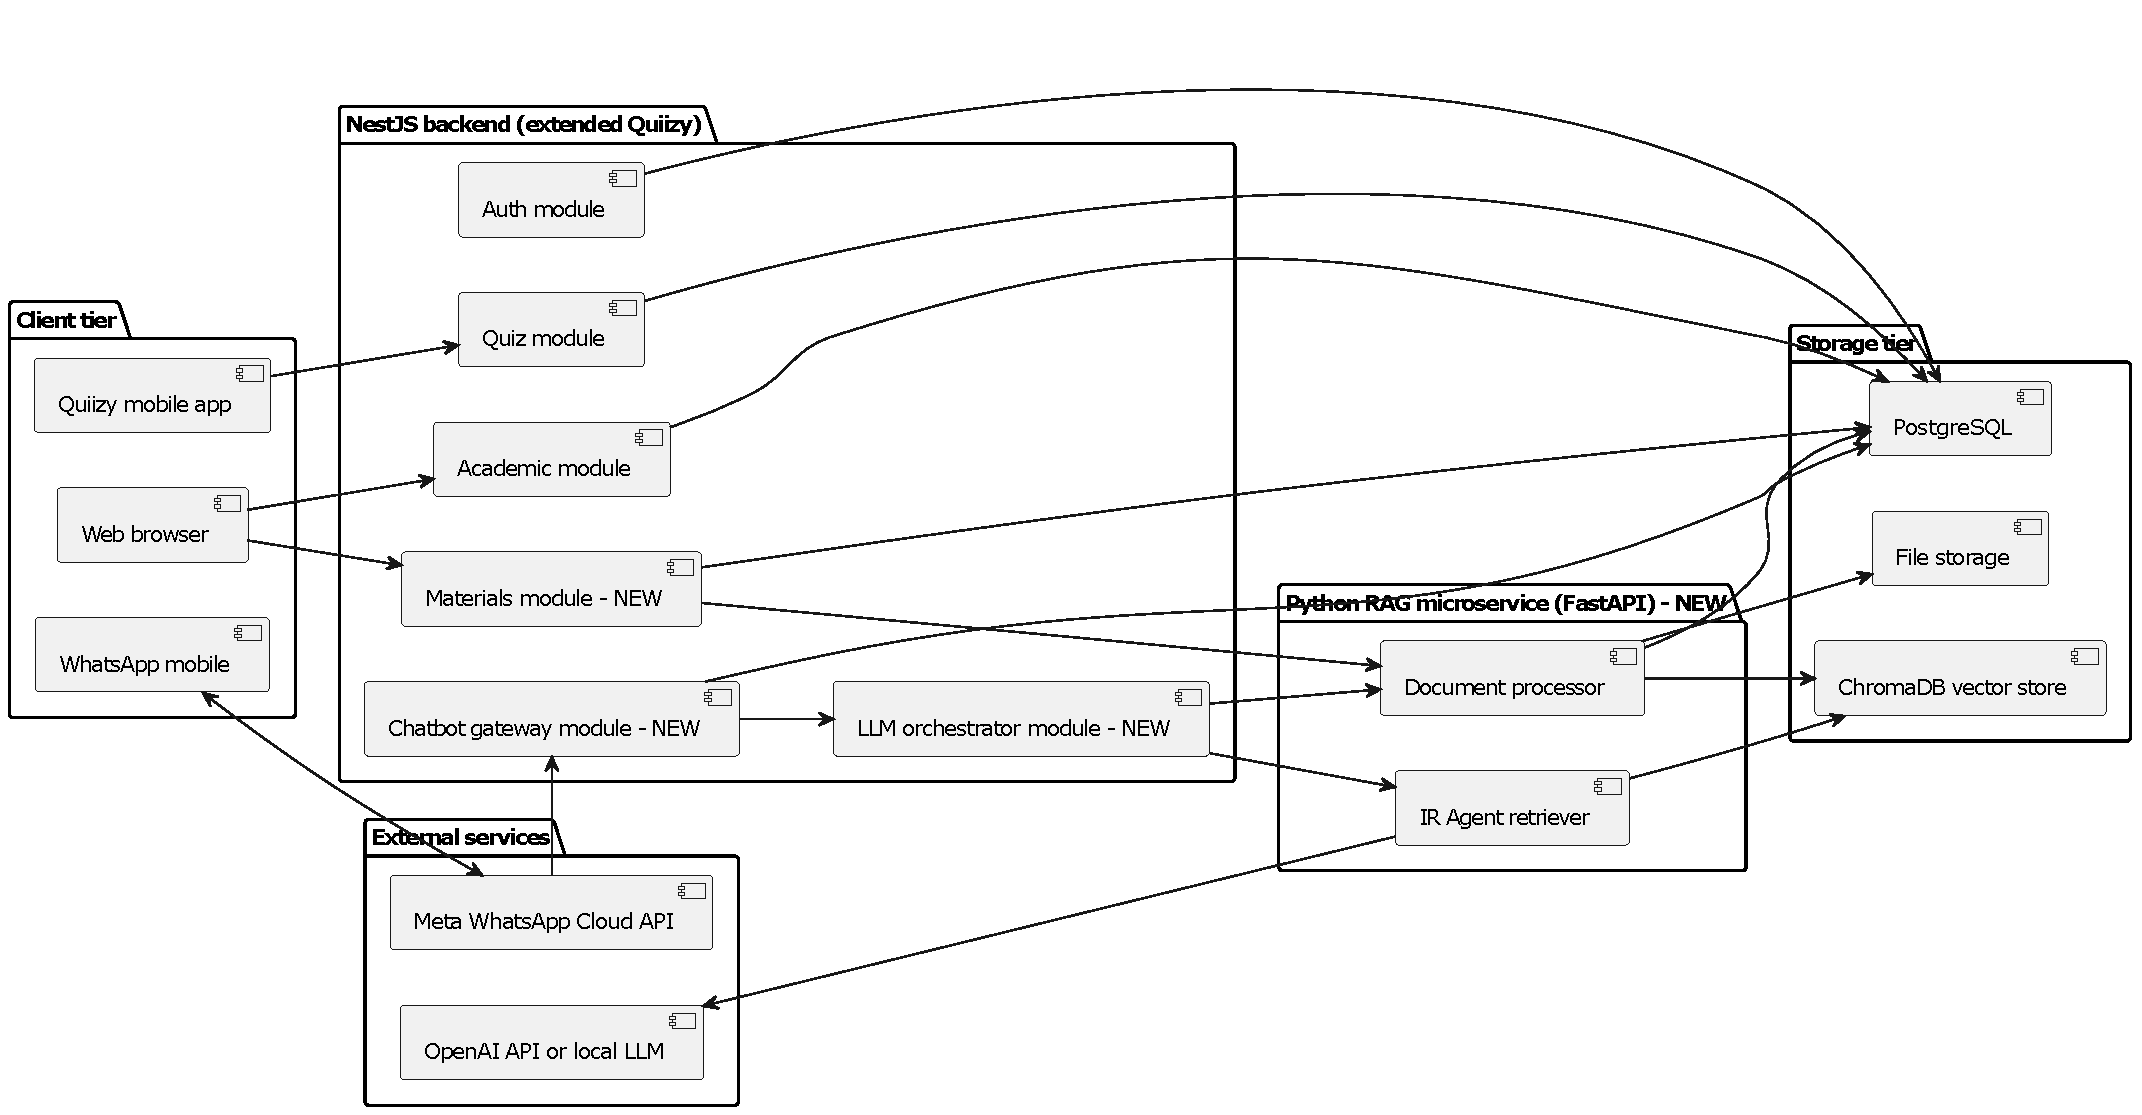
\includegraphics[width=1.06\textwidth]{images/componentDiagram.pdf}
  \caption{Component architecture of the extended Quiizy campus assistant}
  \label{fig:component-architecture}
\end{figure*}

The NestJS backend coordinates the overall workflow. Three new functional
areas are introduced:
\textbf{Materials} (upload, persistence, and processing coordination),
\textbf{Chatbot Gateway} (conversational interface webhook handling and session
management), and an \textbf{LLM Orchestrator} (prompt assembly and
invocation of retrieval and generation).

A separate Python FastAPI service performs the document indexing and
retrieval steps \cite{fastapiDocs}. This separation isolates
language-processing concerns from the core LMS backend and leverages
Python libraries commonly used for text extraction and semantic search.

For semantic retrieval, the system uses ChromaDB as the vector store
\cite{chromaDocs,gao2023retrieval}. Storage is therefore split across:
PostgreSQL (structured LMS data and metadata), file storage (raw uploaded
documents), and ChromaDB (embeddings used for similarity search).

\subsection{MVC Architecture and Processing Pipeline}
\label{sec:model:mvc}

Quiizy follows the standard NestJS structure: controllers receive HTTP
requests, services implement logic, and repositories access the
database. In this project, the AI-related work (document indexing and
retrieval) is handled by the Python service. Figure
\ref{fig:mvc-architecture} summarizes this split.

\begin{figure*}[htbp]
  \centering
  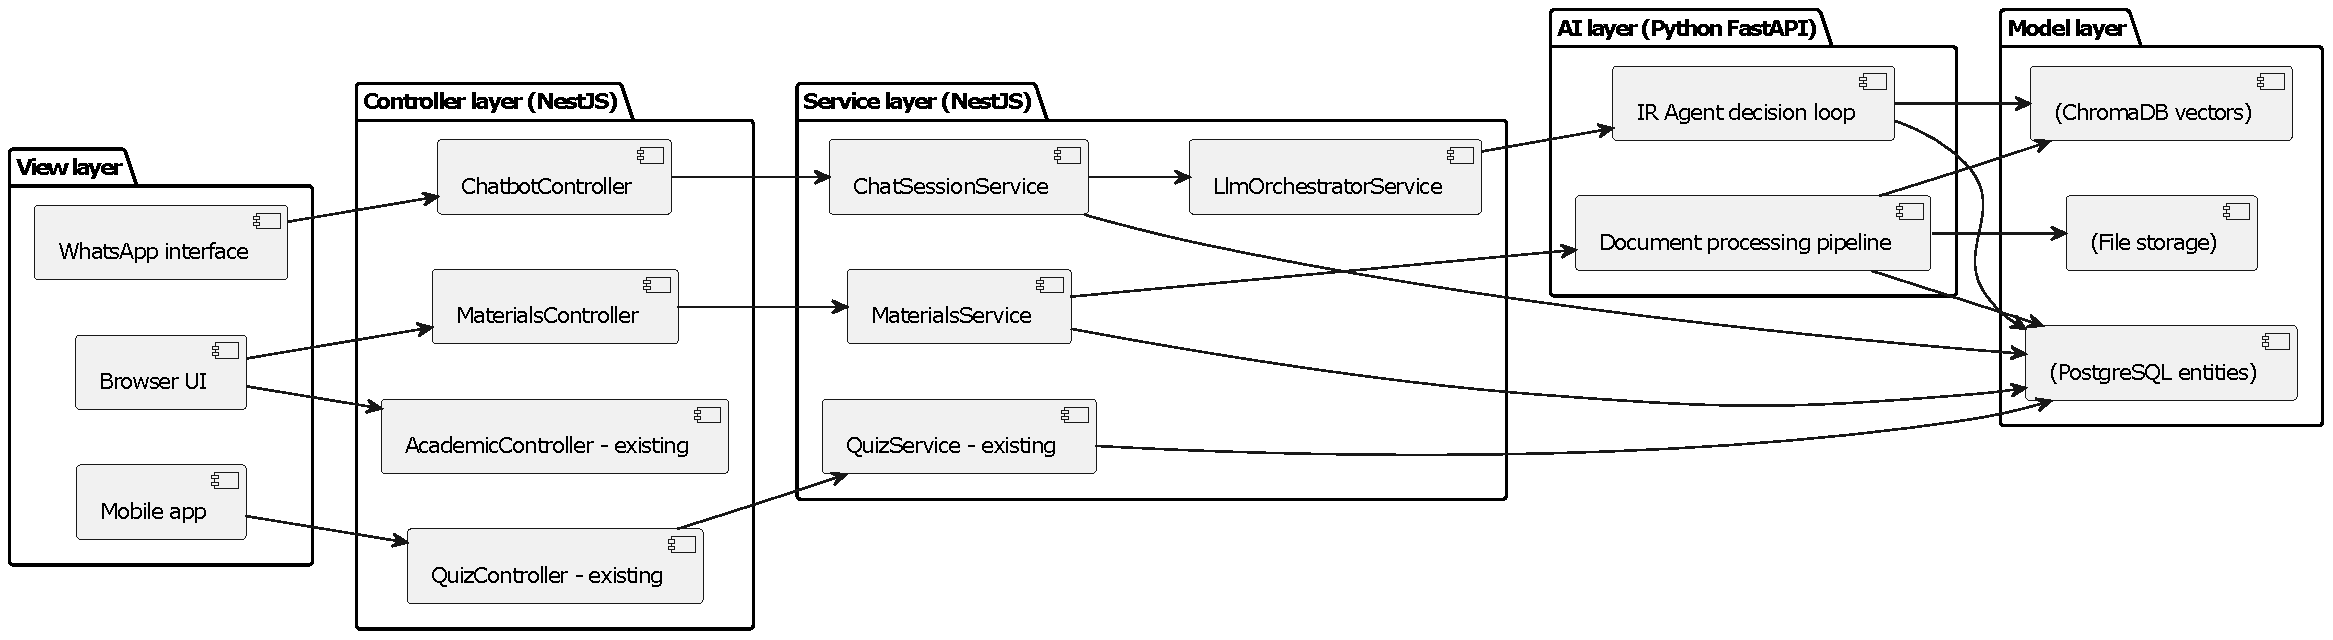
\includegraphics[width=1.06\textwidth]{images/mvc.pdf}
  \caption{Extended MVC architecture showing the AI layer}
  \label{fig:mvc-architecture}
\end{figure*}

At the system boundary, two controllers handle external input:
\texttt{ChatbotController} (conversational chat interface) and \texttt{MaterialsController}
(file upload). Controllers perform request validation and delegate to
services for business logic.

For chat, the service manages a conversation session, associates the
phone number with a student account when possible, and queries the Python
retrieval endpoint for relevant passages. The orchestrator then builds a
prompt that includes conversation context, retrieved passages, and a
language directive, and finally requests the LLM to generate the reply.

For documents, the Python service processes uploads by extracting text,
splitting it into chunks, computing embeddings, and storing them in
ChromaDB. For each query, it embeds the question and retrieves the most
similar chunks as evidence. If retrieval does not return sufficiently
relevant passages, the assistant returns a controlled fallback response
to avoid unsupported statements.

\subsection{Information Model}
\label{sec:model:information}

The information model, shown in Figure \ref{fig:information-model},
extends the existing Quiizy data schema with two new entity groups. The
existing entities for academic structure (\texttt{Course},
\texttt{Semester}, \texttt{ClassAcademicYear}, \texttt{Student},
\texttt{Teacher}) are shown to provide relational context. The new
entities are \texttt{CourseMaterial}, which represents an uploaded
document, and the pair \texttt{ChatSession} and \texttt{ChatMessage},
which together represent a conversational interaction.

\begin{figure*}[htbp]
  \centering
  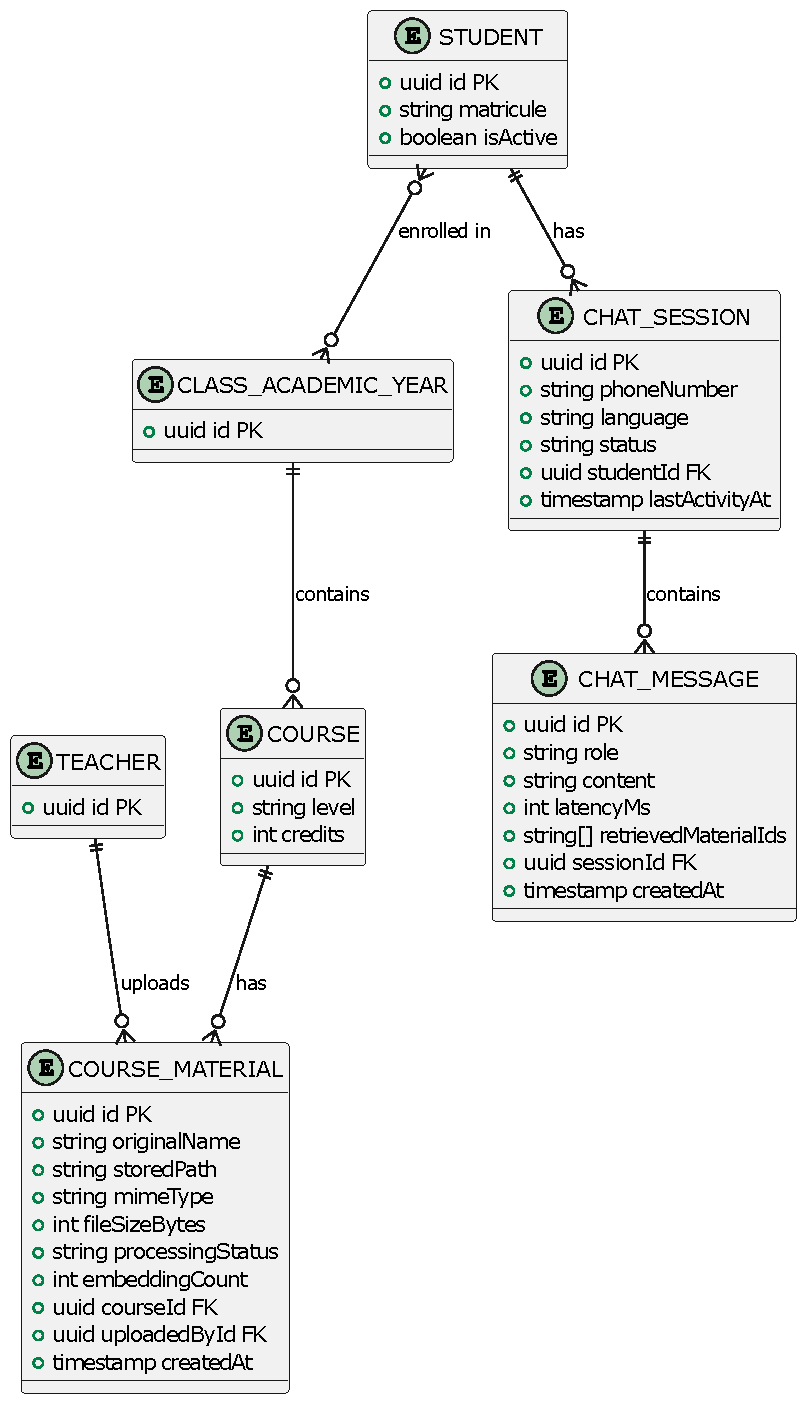
\includegraphics[width=0.88\textwidth]{images/InformationModel.pdf}
  \caption{Extended information model showing new entities in relational context}
  \label{fig:information-model}
\end{figure*}

The central new entity is \texttt{CourseMaterial}, linking an uploaded
file to a course. The \texttt{processingStatus} field tracks the indexing
lifecycle (\texttt{PENDING}, \texttt{PROCESSING}, \texttt{INDEXED},
\texttt{FAILED}), and \texttt{embeddingCount} records how many chunks were
successfully indexed.

Chat interactions are represented by \texttt{ChatSession} and
\texttt{ChatMessage}. Sessions are keyed by a unique session identifier linked
to the student, and can be linked to a \texttt{Student} record to enable
personalization and session history retrieval. Messages store user queries and assistant replies, and can
record which materials contributed to the answer to support traceability.

ChromaDB remains external to the relational ERD: it stores embeddings and
associated identifiers (e.g., \texttt{material\_id}, \texttt{course\_id}) so
retrieved text can be traced back to the originating course document.

\subsection{Technology Choices and Design Rationale}
\label{sec:model:rationale}

The technology choices follow the UCD requirements and the architectural
goal of grounding answers in institutional sources.

\textbf{Student conversational interface.} The design specifies a conversational
interface for students to interact with the assistant via natural dialogue, reducing
onboarding effort compared to menu-driven systems. The original architectural design
considered WhatsApp as a student interface to leverage mobile-first usage patterns and
the Meta WhatsApp Cloud API with webhooks for receiving messages and delivering responses
\cite{metaWhatsAppCloudApi}. However, due to time constraints during implementation, the
team focused on developing a web-based conversational interface that achieves the same
pedagogical and functional goals while enabling rapid iteration. The web interface supports
the same conversational agent architecture and multilingual response generation, preserving
the core design goals without requiring mobile channel integration at this stage. WhatsApp
integration remains a viable extension for future deployment phases.

\textbf{Quiizy backend stack (NestJS, PostgreSQL, TypeORM).} The existing
platform stack is retained to minimise disruption to institutional
workflows. NestJS provides a modular structure for controllers and
services \cite{nestjsDocs}. PostgreSQL is used as the relational data
store for structured academic entities \cite{postgresDocs}, and TypeORM
provides an object-relational mapping layer with support for PostgreSQL
and schema evolution \cite{typeormDocs}.

\textbf{Python retrieval service (FastAPI).} The RAG workflow combines
retrieval and generation \cite{lewis2020retrieval,gao2023retrieval} and
benefits from Python tooling for document processing and embedding-based
search. A separate FastAPI service is therefore used to encapsulate the
indexing and retrieval pipeline behind a stable HTTP interface
\cite{fastapiDocs}. This service boundary aligns with common distributed
deployment practices in cloud-based systems such as AWS, where microservices
architectures enable scalable and maintainable solutions
\cite{shukur2020cloud,rashid2018distributed}.

\textbf{Vector store (ChromaDB).} ChromaDB is used to store embeddings and
metadata and to support similarity-based retrieval \cite{chromaDocs}. It
can be run locally or self-hosted, enabling a lightweight deployment
path, and it matches the vector-store role described in RAG surveys
\cite{gao2023retrieval}.

\textbf{Bilingual interaction.} The assistant responds in the language of
the incoming message (English or French) using a single prompt and a
single LLM endpoint. This avoids maintaining parallel pipelines while
still supporting bilingual access.

The next chapter describes the implementation.

\section{Implementation}
\label{sec:implementation}

This chapter describes the implementation of the proposed Smart Campus AI Assistant, translating the design and modeling presented in Chapter 3 into a working prototype. The implementation is guided by the Nunamaker methodology's System Development phase and specifically addresses research objectives RO1.3--I and RO2.3--I, which call for implementing a bilingual web-based prototype with English and French support for academic service access, deploying it on AWS cloud infrastructure, and instrumenting it for systematic evaluation.

The implementation follows a pragmatic layered architecture that separates concerns across frontend (mobile and web), backend API, and specialized AI services. A key architectural principle is offline-first design: the mobile application maintains a local SQLite database for quiz data and student answers, synchronizes opportunistically with the backend via a sync queue, and remains functional even when network connectivity is intermittent. This approach is essential for the Central African university context where connectivity may be unreliable. The backend services, implemented in NestJS with PostgreSQL, maintain academic structure, authentication, and quiz management. A separate Python FastAPI microservice handles the RAG pipeline, document indexing, and LLM orchestration. Together, these components realize the design requirements while addressing the remaining challenges identified in Chapter 2, particularly RC1 (bilingual context-aware assistants for Central Africa), RC2 (avoiding LLM hallucination through retrieval grounding), and RC4 (platform integration with Quiizy).

\subsection{Backend Services and API Layer}
\label{sec:impl:backend}

The backend is built on NestJS, a Node.js framework that provides a modular, scalable structure aligned with the existing Quiizy platform. The API layer exposes three main functional areas: academic information endpoints, authentication and session management, and quiz and assessment endpoints. All endpoints follow REST conventions and are protected by JWT-based authentication, consistent with the design in Chapter 3.

The academic information service manages the hierarchical structure of the institution: academic years, semesters, classes, courses, and teaching units. These entities map to the information model defined in Section 3.5 and are stored in a PostgreSQL relational database. A request to retrieve the current academic year for a logged-in student, for example, queries the database for the active academic year and returns it as JSON. The service also manages student-class linkages, enabling personalized course and quiz lists. The API is designed to be stateless: each request includes the student's JWT token, which the backend validates and uses to determine the requesting user's role and permissions.

\begin{figure*}[htbp]
  \centering
  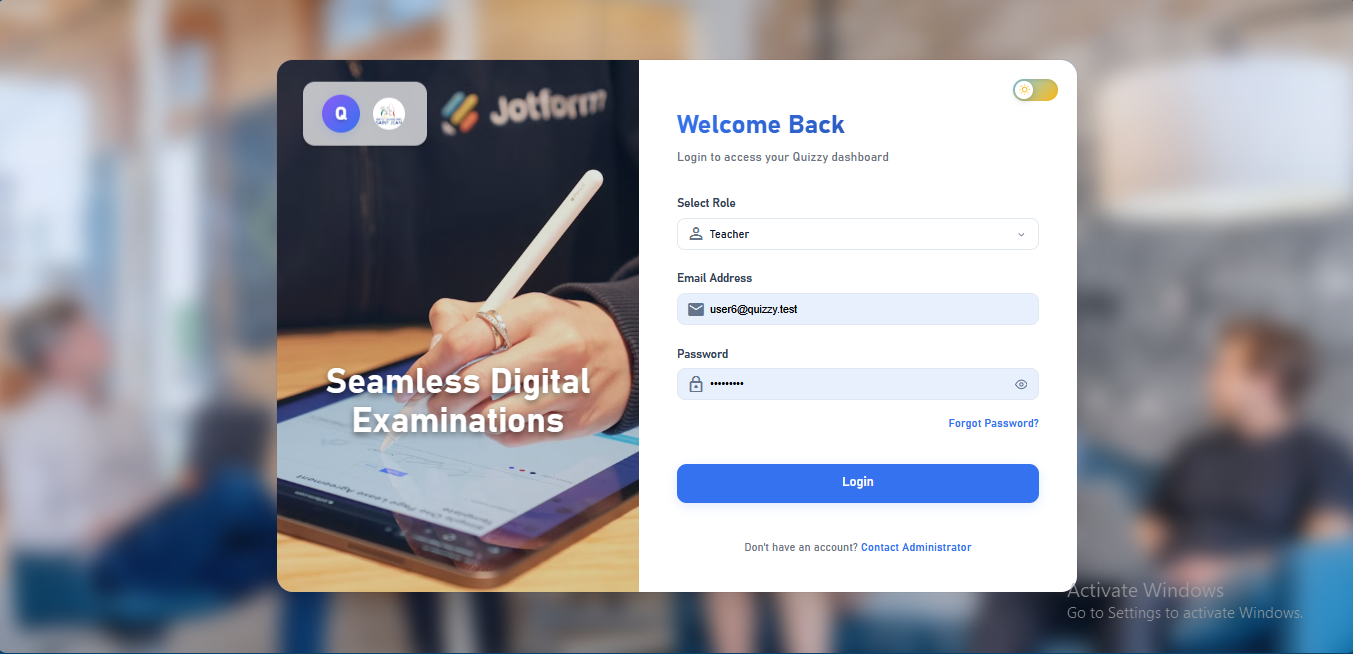
\includegraphics[width=0.95\textwidth]{images/quiizy_login.png}
  \caption{Quiizy login interface: teacher and administrator authentication with role selection}
  \label{fig:quiizy-login}
\end{figure*}

Authentication is implemented via JWT tokens following industry standards. When a student logs in with email and password, the backend validates credentials against a secure password hash, generates a JWT access token with a short expiration time (typically 15 minutes), and returns a refresh token with a longer expiration (typically 7 days). The refresh token is stored securely on the client, allowing the mobile or web application to obtain a new access token when the old one expires, without requiring the user to re-enter credentials. This pattern balances security and user experience.

The quiz service manages the complete lifecycle of assessments: creating quizzes, associating questions, recording student participation, and computing scores. When a quiz is created by a teacher, it is linked to a course and specified with a start time, end time, duration, and question bank. When a student starts a quiz, a student-quiz record is created to track that student's participation, recording the start time and initial participation status. As the student answers questions, each answer is recorded in a student-answer table linked to the student-quiz record. Critically, the backend does not immediately compute or return the mark; instead, it stores the answer and marks the record for synchronization. This allows the mobile client to work offline: answers are queued locally and synchronized when connectivity is restored, as explained below.

The implementation uses TypeORM as the object-relational mapping layer, providing an abstraction over SQL queries and supporting schema migrations. Migration files define schema changes (e.g., adding a new column for question difficulty) in a version-controlled way, allowing the team to maintain consistency across development, staging, and production environments. This is important for an application deployed on AWS, where schema evolution must be coordinated across multiple instances. The web interface for academic administrators manages semesters and teaching units, providing dashboards for creating and configuring core academic structures, as shown in Figures \ref{fig:quiizy-semesters} and \ref{fig:quiizy-teaching-units}.

\begin{figure*}[htbp]
  \centering
  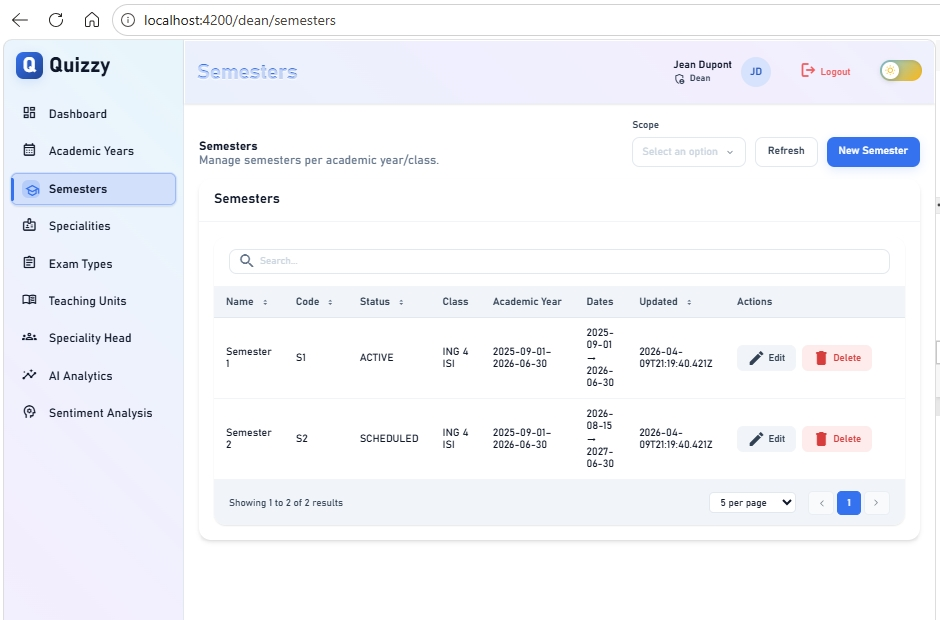
\includegraphics[width=0.95\textwidth]{images/quiizy_semesters.png}
  \caption{Quiizy administration dashboard: semesters management interface for academic year configuration}
  \label{fig:quiizy-semesters}
\end{figure*}

\begin{figure*}[htbp]
  \centering
  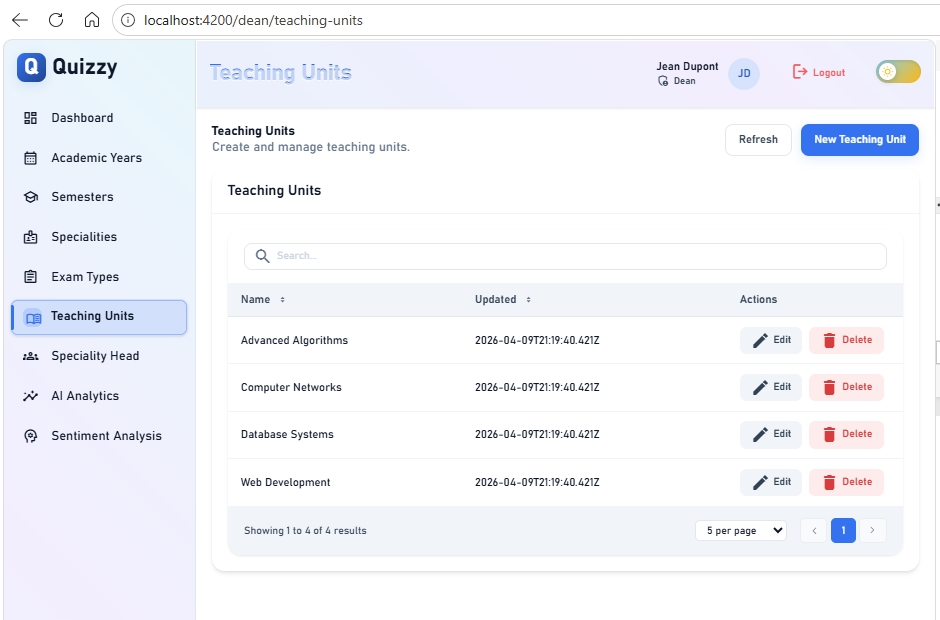
\includegraphics[width=0.95\textwidth]{images/quiizy_teaching_units.png}
  \caption{Quiizy administration dashboard: teaching units management for course organization}
  \label{fig:quiizy-teaching-units}
\end{figure*}

\subsection{Mobile Application: Offline-First Design}
\label{sec:impl:mobile}

The mobile application is implemented in React Native using the Expo framework, targeting both iOS (via Mac build service) and Android. The offline-first architecture is a distinctive aspect of the implementation that directly addresses the infrastructure constraints identified in Chapter 1. Rather than requiring continuous connectivity, the app maintains a complete local copy of relevant academic data in a SQLite database stored on the device.

When the application is launched, it initializes the local database by creating tables matching those defined in the information model: academic years, semesters, courses, quizzes, questions, student answers, and chat sessions. This local copy is populated through a pull-sync operation: the app queries the backend for all courses, quizzes, and academic information relevant to the logged-in student and caches these in the local database. Subsequent quiz interactions---starting a quiz, answering questions, submitting a quiz---operate on this local copy without requiring network I/O. Answers are recorded in the local student-answer table. This pattern ensures that a student can continue taking a quiz even if the Internet connection is lost mid-quiz.

Synchronization is managed through a sync queue: a table in the local SQLite database that records pending operations (e.g., ``start quiz'', ``submit answer'', ``mark quiz complete'') along with their data. A sync manager, running in the background or triggered when connectivity is restored, processes the sync queue: it batches pending operations, sends them to the backend API, and marks them as synchronized once the backend confirms receipt. If a network error occurs during sync, failed items remain in the queue and are retried later. The sync queue implementation is crucial for supporting offline grace periods: the application can operate offline for a defined grace period (currently seven days), allowing students to continue participation even during extended connectivity outages. Listing \ref{lst:sync-queue} illustrates the core sync operation.

\begin{minted}{typescript}
export const addToSyncQueue = async (
  operationType: string,
  entityId: string,
  data?: any
): Promise<void> => {
  const db = await getDatabase();
  const timestamp = new Date().toISOString();
  const isSynced = false;
  const retryCount = 0;
  
  await db.runAsync(
    `INSERT INTO sync_queue 
    (operation_type, entity_id, data, timestamp, retry_count) 
    VALUES (?, ?, ?, ?, ?)`,
    [operationType, entityId, JSON.stringify(data), timestamp, retryCount]
  );
};

export const getPendingSyncItems = async (): Promise<SyncQueueItem[]> => {
  const db = await getDatabase();
  const result = await db.getAllAsync(
    `SELECT * FROM sync_queue WHERE is_synced = 0 ORDER BY timestamp ASC`
  );
  return result as SyncQueueItem[];
};
\end{minted}
\captionof{listing}{Sync queue processing: core operation from syncQueueOperations.ts}
\label{lst:sync-queue}

The notification system on the mobile application uses Expo Notifications, integrating with platform-native notification services (APNs for iOS, FCM for Android). Notifications are scheduled to alert students of upcoming quiz deadlines, deadline changes, and quiz availability. The notification scheduler checks the local quiz database on a daily basis, identifies quizzes that are coming due within a defined window (e.g., 24 hours), and schedules local notifications. The app also stores a notification history in the local database, allowing students to dismiss or revisit notifications without network connectivity.

The mobile UI is organized around a bottom-tab navigation pattern: students navigate between Home (dashboard), Academics (courses and schedules), Exams (quiz list), and Profile. The Exams tab displays all quizzes relevant to the current student, filtered by status (upcoming, in progress, completed). When a student selects a quiz, the app navigates to a detail screen showing the quiz description, deadline, and duration. Tapping ``Start Quiz'' transitions to a quiz-taking screen that displays questions one at a time, records answers locally, and tracks elapsed time. Upon submission, the app computes the grade locally (if grading rules are simple) or queues the submission for backend grading and sync. This pattern ensures smooth interaction even during partial connectivity.

\subsection{Web Application: Teacher and Academic Administrator Dashboard}
\label{sec:impl:web}

The web application is implemented in Angular, following standard single-page application (SPA) architecture. It serves as the interface for teachers and academic administrators to upload course materials, manage quizzes, review student results, and configure system settings. The web app communicates with the backend API via HTTP requests, maintaining authentication via JWT tokens stored in the browser's secure storage.

For teachers, the primary workflow is uploading course materials (lecture notes, slides, reading materials) to be indexed for RAG-based retrieval. The materials upload interface provides a file input accepting PDF, DOCX, and text files. When a teacher selects and uploads a file, the web frontend sends it to the backend, which coordinates with the Python FastAPI service to extract text, split the content into semantic chunks, compute embeddings using a pre-trained language model, and store the embeddings in ChromaDB. The backend returns a processing status (PENDING → PROCESSING → INDEXED or FAILED), allowing teachers to monitor ingestion progress. Listing \ref{lst:material-upload} shows the essential request structure.

\begin{minted}{typescript}
export class TeacherApiService {
  private apiUrl = environment.apiUrl;
  
  uploadCourseMaterial(
    courseId: string,
    file: File,
    materialTitle: string
  ): Observable<{processingStatus: string; materialId: string}> {
    const formData = new FormData();
    formData.append('file', file);
    formData.append('courseId', courseId);
    formData.append('title', materialTitle);
    
    return this.http.post<{processingStatus: string; materialId: string}>(
      `${this.apiUrl}/materials/upload`,
      formData
    );
  }
}
\end{minted}
\captionof{listing}{Course material upload endpoint: Angular service integration}
\label{lst:material-upload}

For academic administrators, the web dashboard provides views of all students, quizzes, and results. An administrator can create new academic years and semesters, link students to classes, and configure system-wide settings such as the offline grace period duration. The dashboard includes charting components displaying quiz participation rates, average scores by course, and student engagement metrics, supporting data-informed decisions about curriculum and support.

The web frontend uses Angular services to encapsulate API calls and state management. A centralized HTTP interceptor, applied to all outbound requests, automatically includes the JWT access token in the Authorization header. A response interceptor detects 401 (Unauthorized) responses, attempts to refresh the access token using the stored refresh token, and retries the original request. If token refresh fails, the interceptor triggers a logout, redirecting the user to the login page. This ensures seamless session management and helps protect against token expiration during a long admin session.

\subsection{Retrieval-Augmented Generation Pipeline}
\label{sec:impl:rag}

The RAG pipeline is implemented as a separate Python FastAPI microservice, decoupled from the NestJS backend. This separation enables independent scaling, technology-appropriate tool choices (Python libraries for NLP and embeddings), and clear service boundaries. The RAG service exposes two main endpoints: one for document ingestion and indexing, and one for retrieval-based question answering.

When a teacher uploads course materials through the web interface, the NestJS backend receives the file, stores it in persistent file storage, and sends a message to the FastAPI service requesting processing. The FastAPI service extracts text from the uploaded file (using libraries such as PyPDF2 for PDFs and python-docx for Word documents), splits the text into semantic chunks using a sliding-window approach (typically 512 tokens per chunk with 128-token overlap to preserve context), and computes embeddings. Embeddings are computed using a pre-trained model (such as OpenAI's text-embedding-3-small or an open-source BERT variant) and stored in ChromaDB along with metadata identifying the source course and material. ChromaDB supports fast similarity search, enabling efficient retrieval of the top-k most relevant chunks given a student question.

When a student sends a question through the chat interface, the question is first passed to the FastAPI retrieval endpoint, which embeds the question and retrieves the top-$k$ (typically $k=3$ or $k=5$) most similar chunks from the vector store. These retrieved chunks, along with the student's question and conversation history, are assembled into a prompt that guides the LLM to generate a grounded answer. The prompt includes a language directive (``Respond in English'' or ``Respond in French'') to enforce the bilingual requirement. For the student chat interface, the implementation uses Google's Gemma-4-31b-it model, deployed through Vertex AI, which generates a response that is returned to the student.

Critically, the RAG approach addresses Remaining Challenge RC2: by grounding the LLM's response in retrieved course materials, the system avoids pure hallucination and ensures that answers are justified by institutional sources. If retrieval returns only low-confidence matches or insufficient relevant passages, the system returns a controlled response such as ``I couldn't find relevant information in the course materials. Please contact the course instructor.'' This fallback prevents unsupported claims. Listing \ref{lst:rag-retrieval} outlines the core retrieval logic.

\begin{minted}{python}
from fastapi import FastAPI
from chromadb import Client as ChromaClient
import openai

app = FastAPI()
chroma_client = ChromaClient()

@app.post("/retrieve")
async def retrieve_and_generate(
    query: str,
    course_id: str,
    language: str = "en",
    top_k: int = 5
):
    # Embed the query
    query_embedding = openai.Embedding.create(
        input=query,
        model="text-embedding-3-small"
    )["data"][0]["embedding"]
    
    # Retrieve from ChromaDB
    results = chroma_client.get_collection(
        name=f"course_{course_id}"
    ).query(
        query_embeddings=[query_embedding],
        n_results=top_k
    )
    
    # Check retrieval confidence
    if not results["distances"][0] or \
       results["distances"][0][0] > SIMILARITY_THRESHOLD:
        return {"answer": "I couldn't find relevant materials."}
    
    # Build context from retrieved chunks
    context = "\n".join(results["documents"][0])
    
    # Generate response via LLM with language directive
    lang_prompt = "English" if language == "en" else "French"
    prompt = f"""Based on the following course material, 
    answer the student question. Respond in {lang_prompt}.
    
COURSE MATERIAL:
{context}

STUDENT QUESTION:
{query}

ANSWER:"""
    
    response = client.models.generate_content(
        model="gemini-2.0-flash",
        contents=prompt
    )
    
    return {"answer": response["choices"][0]["message"]["content"]}
\end{minted}
\captionof{listing}{RAG retrieval endpoint: core function from FastAPI service}
\label{lst:rag-retrieval}

\subsection{Chat Interface Design and RAG Integration}
\label{sec:impl:chat}

While a full WhatsApp Cloud API integration was designed as part of the conceptual architecture, time constraints during implementation necessitated focusing on a web-based chat interface for the student-assistant interaction. This web-based chatbot enables students to interact with the assistant through natural dialogue, demonstrating the feasibility of the conversational assistant concept. The full WhatsApp integration remains a designed component that can be deployed in future iterations without major architectural changes.

The chat interface receives incoming messages, creates or retrieves a chat session identified by the student's unique identifier, and routes the message to the RAG pipeline. The RAG service retrieves relevant course materials and generates a response in the student's preferred language (inferred from message content or stored in user preferences). The response is returned to the student through the web chat interface.

The conversational interface is designed to maintain context across multiple turns within a session, allowing students to ask follow-up questions. For example, a student might ask ``When is the deadline for the data structures quiz?'', receive an answer, and then ask ``How long does it last?'' The system maintains the conversation history in a chat-session database, allowing the LLM to understand the follow-up question in context. This multi-turn support addresses the requirement noted in Chapter 2 that campus assistants should support goal-directed student tasks beyond simple fact retrieval.

\subsection{Cloud Deployment and Infrastructure}
\label{sec:impl:cloud}

The complete prototype is deployed on Amazon Web Services (AWS), leveraging managed services to reduce operational overhead and support scalability. The architecture uses the following AWS components:

\textbf{EC2 for containerized services.} The NestJS backend and Python FastAPI service are containerized using Docker, with container images stored in Amazon ECR (Elastic Container Registry). The services are orchestrated on AWS ECS (Elastic Container Service) using Fargate, a serverless container runtime that eliminates the need to manage EC2 instances. Auto-scaling policies are configured to increase the number of container instances when CPU or memory utilization exceeds a threshold, ensuring responsiveness under variable load.

\textbf{RDS for PostgreSQL database.} The PostgreSQL database is hosted on Amazon RDS (Relational Database Service), which provides automated backups, point-in-time recovery, and failover capabilities. RDS is configured with read replicas for scaling read-heavy workloads such as quiz queries.

\textbf{S3 for file storage.} Uploaded course materials and generated documents are stored in Amazon S3 (Simple Storage Service), which offers high durability, low-cost storage, and direct integration with the application tier. S3 bucket policies are configured to restrict access to authenticated application instances.

\textbf{API Gateway for request routing.} AWS API Gateway provides a managed API endpoint that sits in front of the containerized services, handling request routing, rate limiting, and SSL/TLS termination. This separates the public-facing interface from the application logic.

\textbf{CloudWatch for logging and monitoring.} Application logs from the backend services are streamed to AWS CloudWatch, enabling centralized log analysis, alerting, and debugging. CloudWatch metrics track CPU, memory, request latency, and error rates, informing auto-scaling and alerting policies.

The deployment pipeline is automated: developers push code to a Git repository, triggering a CI/CD pipeline (using AWS CodePipeline and CodeBuild) that runs tests, builds container images, and deploys to ECS. This enables rapid iteration and reduces deployment errors.

\subsection{Bilingual Support: Chat Interface}
\label{sec:impl:bilingual}

Bilingual support is implemented in the chat interface, enabling students to interact with the system in English or French. When a student sends a message through the chat interface, the backend infers the language from the message content using a language detection library (e.g., \texttt{langdetect} in Python) or from the student's stored preference. The language inference is passed to the RAG pipeline, which ensures that the LLM response is generated in the appropriate language.

The RAG pipeline uses a multilingual embedding model (e.g., OpenAI's text-embedding-3-small) that produces embeddings comparable across English and French, enabling effective retrieval regardless of the language of the incoming query or stored materials. For document processing, text is extracted and chunked without language-specific processing, as the multilingual embedding model handles language-agnostic semantic representation. The LLM prompt includes a language directive (``Respond in English'' or ``Respond in French'') to enforce the requested language in the generated response.

\subsection{Addressing Remaining Challenges Through Implementation}
\label{sec:impl:challenges}

The implementation directly addresses the six remaining challenges identified in Chapter 2. RC1 (bilingual Central African assistants) is addressed through the chat interface supporting English and French interaction on a web-based platform. RC2 (avoiding LLM hallucination) is addressed through the RAG pipeline, which grounds all responses in retrieved institutional materials and includes fallback responses when retrieval confidence is low. RC3 (bilingual RAG in African contexts) is addressed through the deployment of a fully functional RAG pipeline in the proposed system. RC4 (platform integration) is addressed through the incorporation of Quiizy academic data into the information model and the use of Quiizy course and quiz structures in the retrieval pipeline. RC5 (combined system requirements) is addressed through the unified implementation combining the chat interface with bilingual support, RAG grounding, and Quiizy integration. RC6 (rigorous evaluation framework) is addressed in Chapter 5, where the implemented prototype is evaluated using the cognitive walkthrough and TAM-based student satisfaction survey.

\subsection{Summary}
\label{sec:impl:summary}

The implementation translates the conceptual design into a working prototype comprising a mobile application with offline-first synchronization, a web dashboard for teacher and admin workflows, a NestJS backend exposing academic data and quiz management APIs, and a Python FastAPI RAG service for document indexing and Gemma-4-31b-it-based question answering. The complete system is deployed on AWS with containerized services, managed databases, and automated CI/CD. Bilingual support is provided through a web-based chat interface for student-assistant interactions, and the offline-first architecture ensures usability in contexts with unreliable connectivity. While WhatsApp integration was designed as part of the conceptual architecture, it could not be implemented due to time constraints during this project phase. The next chapter evaluates this implementation using cognitive walkthrough and student satisfaction assessment grounded in the technology acceptance model.


\section{Evaluation}
\label{sec:evaluation}


\section{Summary and Outlook}


\newpage
\appendix
\printbibliography[heading=bibintoc]
\printglossary[title=Glossary,toctitle=Glossary]

\end{document}
